\section{Introduction}

\subsection{The Rise of Agentic AI}

Agentic artificial intelligence (AI) represents a transformative leap in AI, evolving beyond reactive systems to autonomous, goal-oriented agents capable of learning, adapting, and making independent decisions~\cite{agentic_ai1}. As it presents immense opportunities, its adoption is growing across industries.  This approach centers on building autonomous agents, often powered by large pretrained models, that can reason, plan, and execute complex, multi-step tasks that have traditionally required significant human intervention. Unlike traditional LLMs that only generate outputs upon receiving prompts, Agentic AI systems actively perceive, reason, and act to achieve long-term objectives in dynamic environments. These systems exhibit traits such as planning, memory retention, self-reflection, and tool/action calls—allowing them to function as intelligent agents that iteratively refine their own reasoning processes.

\paragraph{Role of Agentic AI in Software Engineering:}

The future of software engineering—SE 3.0—is already unfolding with the rise of AI teammates: autonomous, goal-driven systems that collaborate with human developers in real-world workflows~\cite{arxiv250715003}. The integration of Agentic AI into Software Engineering marks a fundamental paradigm shift. Intelligent agents can now autonomously navigate software repositories, understand development history, and make informed decisions that traditionally required human judgment~\cite{traceability,btlink}. They can perform code review, refactoring, dependency analysis, and link recovery across complex version-controlled systems. In software engineering, this paradigm offers a powerful new method for automating intricate workflows, particularly in the complex, resource-intensive process of bug management, thus accelerating software evolution.

\subsection{Agentic AI System for Issue Resolution}

Among the many potential applications of Agentic AI in Software Engineering, one of the most impactful is its use in automating bug fixing, in more formal terms issue resolution. We can conceptualize the ideal bug management lifecycle as a three-stage pipeline: Traceability, Explainability, and Resolution.

\begin{enumerate}
    \item \textbf{Traceability:} Detecting and ranking commits that are most relevant to a given issue through a learning-to-rank formulation that captures one-to-many link structures~\cite{r11,r7,r17}. We aim to build a robust traceability layer that can accurately map issues to their corresponding commits, even in complex scenarios where multiple commits address a single issue~\cite{r21}.

    \item \textbf{Explainability:} Providing interpretable reasoning behind each link to enhance trust and support human understanding of software evolution~\cite{r45}. This involves generating natural language explanations that elucidate why specific commits were linked to particular issues, drawing on historical data and contextual information from the repository~\cite{r7}. By making the decision-making process of the traceability agent transparent, we can foster greater confidence in its recommendations and facilitate more effective collaboration between human developers and AI agents.

    \item \textbf{Resolution:} Building an agentic framework that not only identifies and explains links but also proposes candidate fixes or commits based on prior issue–resolution patterns~\cite{r89,r90}. We envision autonomous agents that can suggest code changes, generate patches, or submit fixes to the repository while providing justifications for their actions; prior work such as \textbf{MAGIS}: LLM-Based Multi-Agent Framework for GitHub Issue Resolution illustrates this potential~\cite{magis}.
\end{enumerate}

\noindent
These three steps collectively aim to transform static traceability recovery into an active, self-improving, and context-aware process led by autonomous software agents. An end-to-end agentic system capable of managing this entire pipeline represents a significant long-term goal for the field. However, such a system is critically dependent on the quality of its foundation. Without a robust and accurate Traceability layer, the Explainability and Resolution agents would operate on flawed or incomplete information, undermining their effectiveness.\\

Therefore, this thesis focuses on solving the foundational traceability problem as the essential first step. We address a critical, unsolved gap in this domain: the recovery of one-to-many issue-commit links. Recovering traceability links between issues and commits is a fundamental requirement for effective software maintenance, comprehension, and analytics. Yet, most existing research has restricted the problem to one-to-one mappings, overlooking the common one-to-many scenarios where a single issue is resolved through multiple commits.

\subsection{One-to-Many Issue–Commit Linking}

Recovering traceability links between issues and commits is a foundational requirement for software maintenance, comprehension, and analytics. However, most existing work has been limited to one-to-one mappings, overlooking the frequent one-to-many relationships where a single issue is resolved through multiple commits~\cite{r11,r17,r21}.


\subsubsection*{Definition of Issue–Commit Links}

Among various traceability relationships, issue–commit linking is one of the most practically relevant. It connects issue reports (e.g., bug fixes, feature requests) to specific code commits that resolve them~\cite{r11,issue-commit-llm}. This relationship is vital for understanding software evolution and maintaining the semantic integrity of repositories.

\begin{figure}[H]
    \centering
    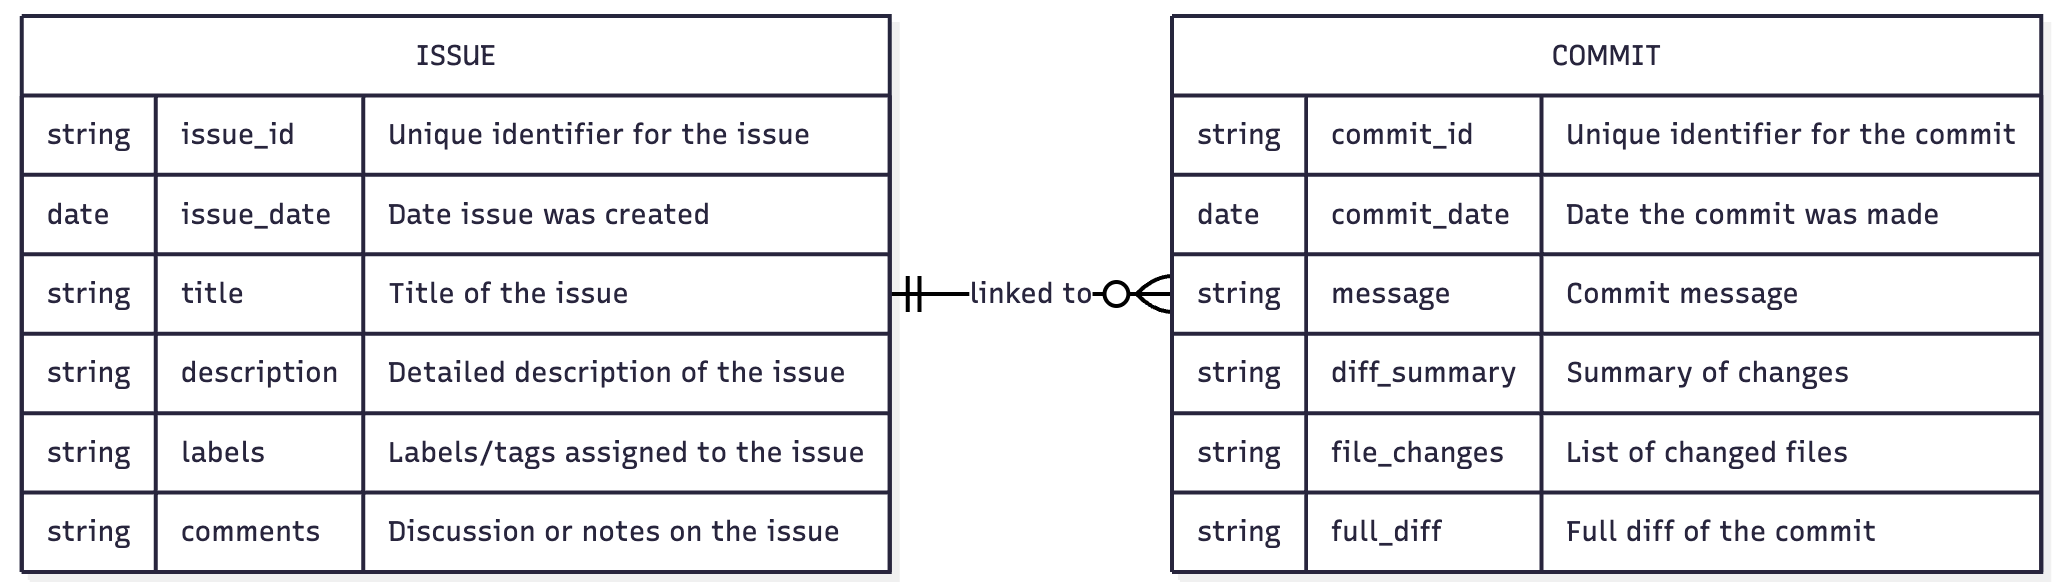
\includegraphics[width=0.98\textwidth]{Figures/er-issue-commit.png}
    \captionsetup{font={small,it},justification=centering}
    \caption{ER model for one-to-many relationship between issues and commits}
    \label{fig:er_issue_commit}
\end{figure}


As shown in Fig.~\ref{fig:er_issue_commit}, each \textit{Issue} entity can be linked to multiple \textit{Commit} entities, capturing the incremental nature of software development where complex issues are often resolved over several commits.


\subsubsection*{Disconnect Between Issue Trackers and Version Control Systems}

A significant challenge in this area arises from the separation between issue tracking systems (e.g., Bugzilla, GitHub) and version control systems (e.g. Mercurial)~\cite{r1,r2}. The lack of integration between the tools results in incomplete traceability hindering maintenance and analytics. Developers may manually include issue IDs in commit messages, but this practice is often inconsistent and error-prone~\cite{r16,r18}, reducing the ability to analyze software changes and understand the rationale behind them. To fill this gap, we present \textbf{LinkRank}, a learning-to-rank formulation for one-to-many issue-commit linking.

\subsection{The \textsc{LinkRank} framework}

Each issue acts as the query, and candidate commits are scored using a compact blend of lexical signals (TF--IDF + SVD) and retrieval focus (BM25), with ranking performed by a LambdaMART model. Selection proceeds via an \emph{iterative pick--remove--renormalize} loop that supports both Known-$K$ and Unknown-$K$ regimes, where $K$ denotes the true number of commits associated with an issue. We also study a complementary commit$\rightarrow$issue variant, \textit{LinkRank-C2I}, that performs bidirectional refinement. \\

\noindent
The remainder of this paper is structured as follows. The Literature Review Section reviews the related work. The Methodology Section introduces the proposed \textsc{LinkRank} framework and its variant \textsc{LinkRank-C2I}, detailing the feature design, LambdaMART training, and selection strategies. The Results Section describes the experimental setup and presents the results across multiple repositories. 

% \bibliographystyle{IEEEtran}
% \bibliography{Reference_Cleaned_IEEE}
